\documentclass[12pt,a4paper]{article}
\usepackage[utf8]{inputenc}
\usepackage[spanish]{babel}
\usepackage{amsmath}
\usepackage{amsfonts}
\usepackage{amssymb}
\usepackage{graphicx}
\usepackage{fancyhdr}
\usepackage{geometry}
\geometry{a4paper,tmargin=1in,bmargin=1in,lmargin=0.6in,rmargin=0.8in} 


% Símbolos de las unidades, sobre todo es para que en una ecuacion no queden en cursiva

\newcommand{\volt}{\mbox{V}}
\newcommand{\mvolt}{\mbox{mV}}
\newcommand{\hertz}{\mbox{Hz}}
\newcommand{\khertz}{\mbox{kHz}}
\newcommand{\Mhertz}{\mbox{MHz}}
\newcommand{\farad}{\mbox{F}}
\newcommand{\nfarad}{\mbox{nF}}
\newcommand{\pfarad}{\mbox{pF}}
\newcommand{\ohm}{\Omega}
\newcommand{\kohm}{\mbox{k}\Omega}
\newcommand{\Mohm}{\mbox{M}\Omega}
\newcommand{\amper}{\mbox{A}}
\newcommand{\mamper}{\mbox{mA}}
\newcommand{\segundo}{\mbox{s}}
\newcommand{\msec}{\mbox{ms}}
\newcommand{\usec}{\mu\mbox{s}}
\newcommand{\nsec}{\mbox{ns}}
\newcommand{\kwatt}{\mbox{kW}}

\providecommand{\E}[1]{\ensuremath{\times 10^{#1}}}
%para que al ir escribiendo se pueda poner \E{potencia} y quede:" x 10^potencia "

%------------------------- Inicio del documento ---------------------------

\begin{document}

%
% Sin cabecera ni pie de página:
%
\thispagestyle{empty}

\begin{figure}[t]
    \centering
    
\includegraphics [scale=0.72]{img/logo_fiuba_alta.jpg}
\end{figure}

\vspace{5.5cm}

\begin{center}
    \Large{Departamento de Electrónica}\\
    \huge{66.10 Circuitos Electrónicos II}\\
    \vspace{.5cm}
    \large{Proyecto: Amplificador de Audio de Potencia Clase G}\\
    \vspace{1cm}
    \begin{tabular}{lc}
    \textbf{Chaure Fernando} & 90389 \\
    \textbf{Combier Natasha} & Intercambio \\    
    \textbf{Marchi Pablo} & 90603 \\
    \textbf{Zurita Francisco} & 89722 \\ 
    \end{tabular}\\
    \vspace{.3cm}
    \small{\today}\\
\end{center}

\vspace{1.5cm}

\begin{center}
\begin{tabular}{|c|c|c|c|}
\hline
Cuatrimestre / Año & 1\sptext{er} cuatrimestre 2012 \\
\hline
Profesores: & Ing. Alberto Bertuccio \\

\hline
\end{tabular}


\vspace{1cm}
\begin{tabular}{|c|c|}
\hline
Fecha de entrega & Firma  \\
\hline
\hspace*{1cm} & \hspace*{3cm}\\
\hline

\hline
\end{tabular}

\vspace{.5cm}

\begin{tabular}{|c|c|c|c|c|}
\hline
\,Nota\, &\multicolumn{3}{|c|}{Fecha de aprobación} & Firma  \\
\hline
\hspace*{1.7cm} & \hspace*{1cm}& \hspace*{1cm} & \hspace*{1cm}  & \hspace*{3cm}\\
\hline
\end{tabular}

\vspace{1cm}
Obsevaciones:
\hrulefill\par
\vspace{.3cm}
\hrulefill\par
\vspace{.3cm}
\hrulefill\par
\vspace{.3cm}
\hrulefill\par
\vspace{.3cm}
\hrulefill\par
\vspace{.3cm}


\end{center}


\newpage
\thispagestyle{empty}
\tableofcontents
\newpage


%estilo de pie y encabezado de pagina
\pagestyle{fancy}
\lhead{66.10 Circuitos Electrónicos 2}
\fancyfoot[C]{1\sptext{er} cuatrimestre 2012}
\setcounter{page}{1}
\fancyfoot[R]{\thepage}


%\input{cada parte del tp}

\section{Introducción}
\section{Objetivos}


\section{Desarrollo}

\subsection{Cálculos del Amplificador de Audio}

\subsection{Cálculos de las Fuentes de Alimentación}

\subsection{Simulaciones}

\subsection{Realización del Circuito Impreso}
\subsection{Realización del Circuito Impreso}
\bigskip 
\subsubsection{Criterios de Diseño}

A la hora de la implementación de los circuitos, se tomaron en cuenta las siguientes reglas de diseño:
\begin{itemize}
\bigskip 

\item Se cuidó que los caminos de los conductores de alimentación sean suficientemente anchos para reducir la resistividad parásita y que estén dispuestos uno próximo al otro, con el objetivo de disminuir el campo eléctrico generado por ellos.

\item Para el cálculo de los capacitores de desacople tuvimos en cuenta el ancho de banda con el que estábamos trabajando, de modo que funcionen a la frecuencia correspondiente y presenten poca impedancia.

\item Se trató de hacer lo mas cortos y eficientes posibles los recorridos de los caminos de señal, para poder reducir la interferencia con los demás elementos del circuito.

\item Conexiones de masas, alimentación y señal sin lazos cerrados, con el objeto de no concatenar ruido.

\item Las líneas de señal y masa se separaron lo máximo posible para reducir las capacitancias parásitas.

\item Las masas de alimentación y del camino de señal se separaron para que el ruido de la línea no contamine la señal. Solo se unen en un punto.

\item Disipadores en el borde de la placa para facilitar instalación y optimizar la disipación de calor.

\item La señal de realimentación se cuidó de no tomarla inmediatamente del nodo donde convergen las corrientes de salida, sino de un punto que tiene la misma tensión pero no circulan corrientes tan altas, para minimizar el ruido y la distorsión por toma de realimentación.

\end{itemize}

\subsubsection*{Distribución general}
La ubicación de los elementos del circuito respeta lo mejor posible las etapas originales del amplificador de potencia. Ésto facilita el seguimiento visual de los componentes y permite detectar fallas mas rápidamente.
Los caminos de los conductores de alimentación se hicieron los suficientemente anchos y dispuestos uno próximo al otro. Al estar cerca los caminos positivos y los negativos y no rodear el circuito, su campo eléctrico no afecta al resto de los componentes.
También se realizó un plano de masa en forma de estrella, para no concatenar ruido, con una parte dedicada a la entrada y la otra a la salida. Esto permite disminuir el ruido y proteger la señal de entrada.



\subsubsection*{Resistencias emisor de salida}
Estas dos resistencias son de baja R y es importante que no se vean muy alteradas. Para evitar el cambio de temperatura hemos cuidado a que ninguna pista pasa debajo de estas dos resistencias. Además, los caminos que las conectan con la salida son anchos y perfectamente simétricos. De ésta forma, las pistas no sólo incorporan poca resistencia en serie sino que además, la incorporan en igual magnitud, cuestión de no perder la simetría a la salida, y que la degeneración de los transistores de salida sea lo mas simétrica posible.

\subsubsection{Disipadores}
\bigskip
Sabiendo que:
$$
   \theta_{ja}=\dfrac{T_{jm}-T_a}{P_D}
$$
$$
	\theta_{ja}=\theta_{jc}+\theta_{cs}+\theta_{sa}
$$

En la cual $\theta_{ja}$ es la resistencia térmica juntura-ambiente. Para cada transistor que maneje altas corrientes se calcula el valor del disipador requerido teniendo en cuenta la potencia disipada y su resistencia térmica. En el caso del transistor del multiplicador $V_{be}$, que requiere estar a la misma temperatura que los de la salida clase B, se ubicará en el mismo disipador para evitar el embalamiento térmico.

\subsubsection{Circuito Implementado}

En la Figura 26 se puede observar el circuito impreso realizado para el amplificador. Son indicadas las entradas y la salida de señal y los bornes de la alimentación.

\begin{figure}[H]
\centerline{
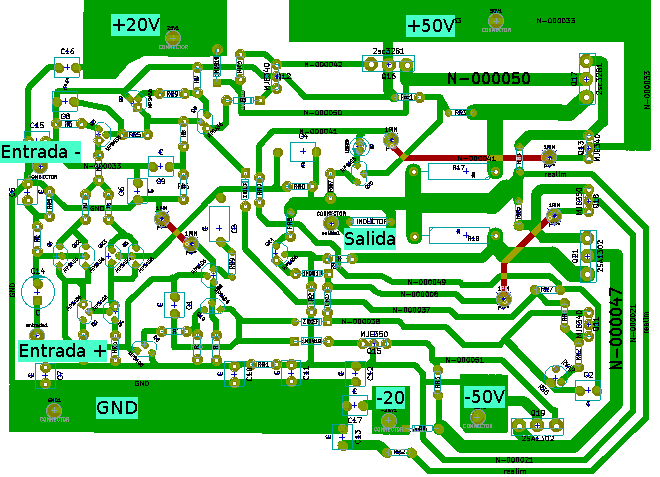
\includegraphics[width=1\textwidth]
{img/PCB1.png}}
\caption{Circuito impreso del amplificador.}
\end{figure}

\subsubsection{Fuente Lineal}
\medskip
Para este circuito se utilizaron pistas de 4mm de ancho. Los diodos utilizados en el puente son 6A10 los cuales pueden soportar las corrientes requeridas por el amplificador, ya que soportan hasta 6A; y poseen una caída de tension en directa menor a 1V.
En la Figura~\ref{circuito_impreso_fuente_lineal} se muestra el circuito impreso implementado. 



\begin{figure}[H]
\centering
\centerline{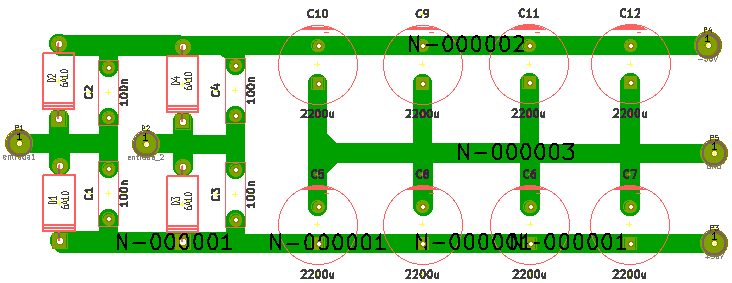
\includegraphics[width=1\textwidth]{img/circuito_impreso_fuente_lineal.png}}
\caption{Circuito impreso de la fuente lineal.}
\label{circuito_impreso_fuente_lineal} 
\end{figure}
\medskip
\subsubsection{Preamplificador}

En este impreso se debió tener en cuenta las posiciones y sentido de giro de los potenciometros para lograr un frente coherente y ordenado. Se agrego un conector jack a la salida para facilitar la desconexión con el amplificador de potencia de ser necesario.
Se utilizaron amplificadores operacionales NE5532, típicos en este tipo de aplicaciones debido a sus buenas prestaciones y bajo ruido.

\begin{figure}[H]
\centering
\centerline{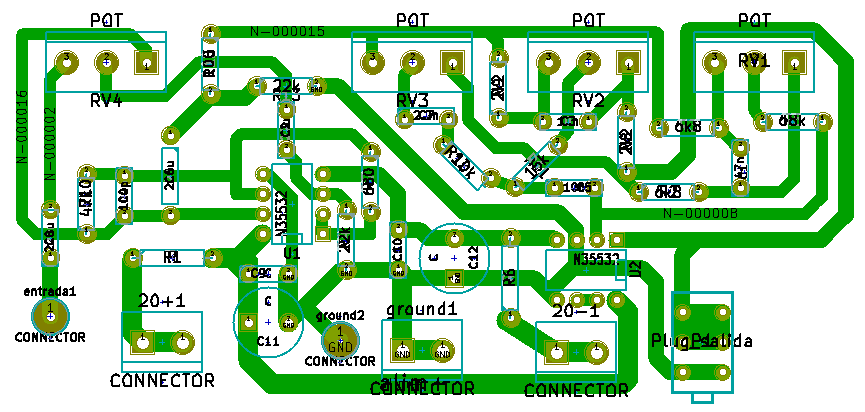
\includegraphics[width=1\textwidth]{img/pre_pcb.png}}
\caption{Circuito impreso del preamplificador.}
\label{pre_pcb} 
\end{figure}

\subsection{Mediciones}

\subsection{Comparativa Mediciones-Simulaciones}

\section{Conclusiones}

\section{Anexos}


\end{document}

